\bookchapter{Capítulo 60: Preparar el entorno de desarrollo: Xcode y el primer proyecto}

\chapterintro{Para hacer bien el trabajo, primero afila tus herramientas. En este capítulo montaremos la “cocina”: instalaremos Xcode, haremos funcionar el simulador, crearemos el primer proyecto iOS de tu vida y desmenuzaremos la estructura del proyecto hasta entenderla. Con el entorno listo, verás por primera vez cómo tu código se convierte en un botón que puedes pulsar; ese instante mucha gente lo recuerda toda la vida.}

\booksection{Consigue un Mac}

Empecemos por el requisito: el desarrollo iOS debe hacerse sobre macOS. Si no tienes Mac, hay tres opciones: comprar uno (un Mac mini o un MacBook Air de segunda mano bastan), alquilar un Mac en la nube a corto plazo, o leer primero la octava parte, “Desarrollo Android en la práctica” (se puede con Windows).

\begin{center}
\begin{tabularx}{\linewidth}{|X|X|X|}
\hline
\textbf{Componente} & \textbf{Mínimo} & \textbf{Zona cómoda (recomendado)} \tabularnewline
\hline
Chip & Apple Silicon (M1 o superior) & M2 o más nuevo \tabularnewline
Memoria & 8GB & 16GB \tabularnewline
Disco & Reservar 40 GB o más (Xcode ocupa mucho) & Desde 256 GB \tabularnewline
Sistema & El macOS más reciente & Mantener las actualizaciones automáticas \tabularnewline
\hline
\end{tabularx}
\end{center}

\begin{center}\small\color{gray}Referencia de configuración de un Mac de desarrollo (agosto de 2026)\end{center}

\begin{tcbinfo}{Consejo: sin Mac también puedes empezar con el lenguaje}
La app gratuita Swift Playgrounds en el iPad permite aprender lo básico de Swift (sin Mac); incluso se puede instalar en el iPhone. Practica en Playgrounds el lenguaje del capítulo 61 y, cuando tengas tu Mac, despega directo. Afilar el hacha no retrasa la tala: de eso se trata.

\end{tcbinfo}

\booksection{Instalar Xcode}

Xcode es el entorno de desarrollo integrado oficial de Apple, y es gratis. Se instala en tres pasos:

\begin{enumerate}
  \item Abre el App Store en el Mac, busca "Xcode" y pulsa instalar; ojo, pesa varios GB, así que elige una franja con buena conexión;
  \item Al abrirlo por primera vez tras la instalación, acepta el acuerdo y deja que se instalen los componentes (se hace solo);
  \item En el menú Xcode Settings Locations, comprueba que Command Line Tools esté seleccionado; las herramientas de línea de comandos son requisito de muchos scripts y herramientas de terceros.
\end{enumerate}

\begin{tcbwarn}{Atención: el juego de emparejar versión y sistema}
El Xcode nuevo suele exigir el macOS más reciente, y los Mac viejos se quedan atascados en versiones antiguas. Para publicar en el App Store, Apple exige compilar con un Xcode relativamente nuevo (suele dar un plazo de gracia). Así que no demores demasiado las actualizaciones del sistema: los desarrolladores iOS son de los que con más puntualidad siguen las versiones nuevas.

\end{tcbwarn}

\booksection{Crea tu primer proyecto}

Abre Xcode Create New Project elige iOS plantilla App, y luego rellena:

\begin{center}
\begin{tabularx}{\linewidth}{|X|X|X|}
\hline
\textbf{Campo} & \textbf{Qué rellenar} & \textbf{Explicación} \tabularnewline
\hline
Product Name & MyFirstApp & Nombre de la app \tabularnewline
Team & Tu Apple ID (gratuito) & Para la firma; con una cuenta personal basta \tabularnewline
Organization Identifier & com.example & Se combina con el Product Name para formar el identificador del paquete \tabularnewline
Interface & SwiftUI & El framework eje de este libro \tabularnewline
Language & Swift & No necesita explicación \tabularnewline
\hline
\end{tabularx}
\end{center}

\begin{center}\small\color{gray}Los cinco campos al crear un proyecto\end{center}

Al pulsar Create, Xcode genera un proyecto que corre directamente. Elige un simulador arriba a la izquierda (por ejemplo, iPhone 17) y pulsa > para ejecutar: a los pocos segundos, en la pantalla del simulador aparece una ventana con el texto “Hello, world!”. Tu primera App iOS acaba de nacer.

\booksection{Anatomía del proyecto: para qué sirve cada archivo}

A la izquierda está el navegador del proyecto; como principiante solo necesitas conocer estos:

\begin{center}
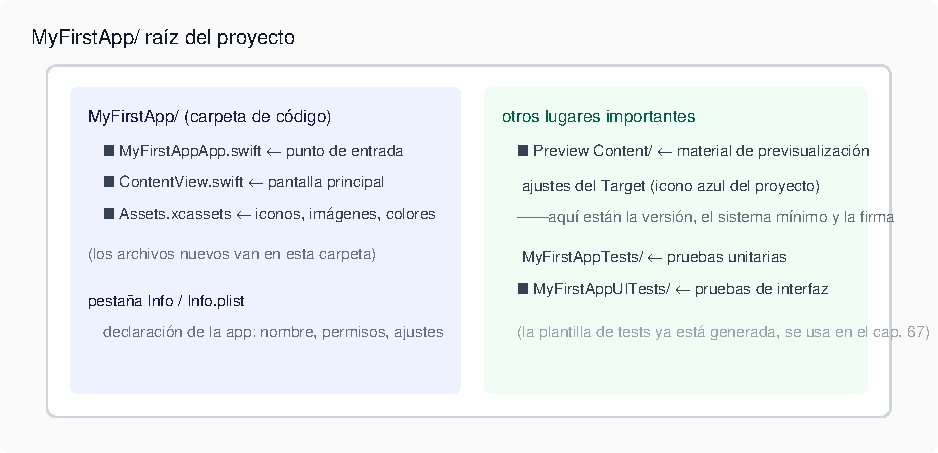
\includegraphics[width=0.92\linewidth]{figures/fig-di-liu-shi-zhang-1}
\\[2pt]\small Figura 2: la estructura de un proyecto Xcode que todo principiante debe conocer
\end{center}

\begin{itemize}
  \item MyFirstAppApp.swift: el punto de entrada del programa; en SwiftUI tiene solo unas líneas: "arranca y muestra la pantalla principal";
  \item ContentView.swift: la vista de la pantalla principal; todo lo que ves ahora vive aquí;
  \item Assets.xcassets: el almacén de recursos; iconos, imágenes y colores van aquí;
  \item Ajustes del Target: entra con el icono azul del proyecto a la izquierda; ahí están el número de versión, la versión mínima de iOS y la firma. El nombre visible de la App y el icono también se configuran aquí.
\end{itemize}

\booksection{Depurar en un dispositivo real: instalar la App en tu iPhone}

\booksection{Trucos de eficiencia en Xcode: los cinco “power-ups” de atajos para principiantes}

Dominando estos parecerás “muy profesional”:

\begin{center}
\begin{tabularx}{\linewidth}{|X|X|X|}
\hline
\textbf{Acción} & \textbf{Atajo} & \textbf{Función} \tabularnewline
\hline
Ejecutar & CmdR & Compilar y arrancar \tabularnewline
Abrir o alternar la vista previa del canvas & OptionCmd & El interruptor del "lo que ves es lo que obtienes" \tabularnewline
Formatear la sangría & CtrlI & Reordena automáticamente la sangría del código seleccionado \tabularnewline
Abrir archivos rápido & CmdO & Escribe el nombre del archivo y se abre al instante (¡el más usado!) \tabularnewline
Comentar o quitar comentarios & Cmd/ & Activar o desactivar código al vuelo mientras depuras \tabularnewline
\hline
\end{tabularx}
\end{center}

\begin{center}\small\color{gray}Atajos de Xcode de uso frecuente (el kit de cinco del principiante)\end{center}

Dos regalos ocultos más: varios simuladores a la vez (ejecutar iPhone e iPad al mismo tiempo para comparar diseños) y la biblioteca de fragmentos de código (arrastra esas líneas que usas mucho al panel Snippets de la derecha y la próxima vez insértalas con un clic); usa primero las herramientas de eficiencia y la soltura llega sola.

\booksection{Depurar en un dispositivo real: instalar la App en tu iPhone}

El simulador está bien, pero el dispositivo real es la meta. Con un Apple ID gratuito también puedes depurar en un móvil real:

\begin{enumerate}
  \item Conecta el iPhone con el cable de datos (o depura por Wi-Fi en la misma red);
  \item En la lista de dispositivos de la parte superior de Xcode elige tu móvil; la primera vez pedirá iniciar sesión con tu Apple ID y configurará la firma automáticamente;
  \item En el iPhone: [Ajustes] [General] [VPN y gestión de dispositivos] confía en tu certificado de desarrollador;
  \item Pulsa > y la App se instala en el dispositivo real.
\end{enumerate}

\begin{tcbwarn}{Atención: la "limitación de siete días" de la cuenta gratuita}
Las Apps firmadas con un Apple ID gratuito caducan a los 7 días (basta volver a ejecutar una vez para renovarlas). Es el mecanismo de Apple contra el abuso, y para aprender sobra; la cuenta de desarrollador de pago (99 USD al año) no tiene esta limitación, como se detalla en el capítulo 67.

\end{tcbwarn}

\booksection{Primera prueba + primeros auxilios para errores comunes}

\booksection{Primera prueba + primeros auxilios para errores comunes}

Abre ContentView.swift, cambia el texto de Text(“Hello, world!”) por tu nombre y pulsa CmdR para volver a ejecutar: a los pocos segundos tu nombre aparece en el simulador. Enhorabuena: acabas de completar tu primer ciclo completo de “cambiar código compilar instalar ejecutar”.

\begin{center}
\begin{tabularx}{\linewidth}{|X|X|X|}
\hline
\textbf{Síntoma del error} & \textbf{Causa habitual} & \textbf{Remedio} \tabularnewline
\hline
Error de Signing & Team sin elegir o certificado caducado & En Target Signing, marca tu cuenta; con cuenta gratuita, vuelve a ejecutar una vez \tabularnewline
El simulador se queda en negro o no abre & Imagen dañada & Menú Device Erase All Content; o borra el simulador y vuelve a añadirlo \tabularnewline
Xcode descarga lento o no se instala & Inestabilidad de red del App Store & Cambia de franja horaria; o descarga el paquete .xip desde el sitio de desarrolladores de Apple \tabularnewline
\hline
\end{tabularx}
\end{center}

\begin{center}\small\color{gray}Tabla de primeros auxilios para errores de entorno del principiante\end{center}

\begin{tcbpractice}{Manos a la obra: completa tu lista de "ritos de desarrollador"}
(1) Instala Xcode y haz funcionar el simulador; (2) ejecuta tu App una vez en un dispositivo real y guarda la captura como recuerdo; (3) cambia el texto de Hello por tu nombre; (4) en los ajustes del Target, cambia el nombre visible de la App a “Mi primera App”. Con estos cuatro pasos, ya eres alguien con una obra propia.

\end{tcbpractice}

\begin{tcbsummary}{Resumen del capítulo}
\begin{itemize}
  \item Requisito duro: Mac + Xcode; sin Mac, empieza aprendiendo el lenguaje con Swift Playgrounds en el iPad
  \item Xcode se instala desde el App Store; las versiones nuevas exigen sistemas nuevos, no demores las actualizaciones
  \item Los cinco elementos al crear un proyecto: nombre, Team, identificador de organización, SwiftUI y Swift
  \item La regla del proyecto: el código vive en la carpeta MyFirstApp/; los ajustes del Target gestionan versión y firma
  \item La depuración en dispositivo real con Apple ID gratuito tiene el límite de firma de 7 días; la cuenta de pago no tiene esa restricción
  \item La rutina de desarrollo = cambiar código CmdR ver el resultado, en bucle
\end{itemize}

\end{tcbsummary}
